% % % % % % % % % % % % % % % % % % % % % % % % % % % % % % % %
% import configuration
% % % % % % % % % % % % % % % % % % % % % % % % % % % % % % % %

% % % % % % % % % % % % % % % % % % % % % % % % % % % % % % % %
% Konfiguration
% % % % % % % % % % % % % % % % % % % % % % % % % % % % % % % %
\newcommand{\titleinfo}{Requirements Specification}
\newcommand{\subjectinfo}{Fleet Monitoring System}
\newcommand{\authorinfo}{Florian Baumgartner, Luca Jost}
\newcommand{\versioninfo}{0.1}
\newcommand{\docNr}{SA FleetMonitor}
\newcommand{\dateinfo}{\today}

% Notes for SRS completion, uncomment the following command to suppress this output
\newcommand{\note}[1]{%
    \vspace{0.25cm}%
    \colorbox{grey}{%
        \parbox{\linewidth-6pt}{%
            \vspace{0.5cm}%
            \centering%
            \parbox{\linewidth-1cm}{%
                \footnotesize{#1}%
            }%
            \vspace{0.5cm}%
        }%
    }%
    \vspace{0.25cm}}
%\newcommand{\note}[1]{}

% % % % % % % % % % % % % % % % % % % % % % % % % % % % % % % %
% Packages, Layout, Units, etc.
% % % % % % % % % % % % % % % % % % % % % % % % % % % % % % % %
%%%%%%%%%%%%%%%%%%%%%%%%%%%%%%%%%%%%%%%%%%
% Dokument
%%%%%%%%%%%%%%%%%%%%%%%%%%%%%%%%%%%%%%%%%%
% Geometrie
\newcommand{\paperFormat}{a4paper}
\newcommand{\lPageMargin}{25mm}
\newcommand{\rPageMargin}{20mm}
\newcommand{\tPageMargin}{20mm}
\newcommand{\bPageMargin}{20mm}

\documentclass[11pt,oneside]{scrartcl}

\newcommand{\newpar}{\par\par}

\usepackage[pdftitle={\titleinfo},%
			pdfauthor={\authorinfo},%
			pdfcreator={pdfLatex, LaTeX with hyperref},
			pdfsubject={\subjectinfo},
			plainpages=false,
			pdfpagelabels,
			colorlinks,
			linkcolor=black,
			filecolor=black,
			citecolor=black,
			urlcolor=black]{hyperref}
			
\usepackage[scaled]{helvet}
%\renewcommand\familydefault{\sfdefault} 


% Headings
\usepackage{scrlayer-scrpage}

%%%%%%%%%%%%%%%%%%%%%%%%%%%%%%%%%%%%%%%%%%
% Package's
%%%%%%%%%%%%%%%%%%%%%%%%%%%%%%%%%%%%%%%%%%
\usepackage[acronym]{glossaries}

\usepackage[OT1]{fontenc}

\usepackage[utf8]{inputenc}

\usepackage[free-standing-units=true,use-xspace=true]{siunitx}

\usepackage{layout}
\setlength{\parindent}{0em}

\renewcommand{\baselinestretch}{1.2}
\renewcommand{\arraystretch}{1}
\newcolumntype{P}[1]{>{\centering\arraybackslash}p{#1}}

%% This changes default fonts for both text and math mode to use Herman Zapfs
%% excellent Palatino font.  Do not change this.
%\usepackage[sc]{mathpazo}

%% The AMS-LaTeX extensions for mathematical typesetting.  Do not
%% remove.
\usepackage{amsmath,amssymb,amsfonts,mathrsfs}

\usepackage[capitalize, noabbrev]{cleveref}	%cref starts with capital letter
\usepackage[usenames,dvipsnames]{pstricks}
\usepackage{setspace}
\usepackage{epsfig}
\usepackage{pst-pdf}
\usepackage{pst-all}
\usepackage{pstricks-add}
\usepackage{supertabular}
\usepackage[font=small,labelfont=bf]{caption}
\usepackage[font=footnotesize]{subfig}
\usepackage{footnote}
\usepackage{float}
\usepackage{multirow}
\usepackage{pdfpages}
\usepackage{pgf,tikz}
\usepackage{color}
\usepackage{titletoc}

\usepackage[makeroom]{cancel}
\usepackage{array}
\usepackage{trfsigns}
\usepackage{textcomp}
\usepackage{booktabs}
\usepackage{rotating}

\usepackage{listings}

\usepackage{tabto}
\renewcommand{\captionfont}{\scriptsize\slshape}

%Inhaltsverzeichnis
\setcounter{secnumdepth}{4}
\setcounter{tocdepth}{2}

%Geometrie
\usepackage[\paperFormat,left=\lPageMargin,right=\rPageMargin,top=\tPageMargin,bottom=\bPageMargin,includeheadfoot]{geometry}

\usepackage{lipsum}%dummy text only
\usepackage{tikz}
\usetikzlibrary{fadings}
\newcommand{\gradient}{\noindent%
    \begin{tikzpicture}
    \fill[black,path fading=west] (-0.5\linewidth,0) rectangle (0,0.1ex);
    \fill[black,path fading=east] (0,0) rectangle (0.5\linewidth,0.1ex);
    \end{tikzpicture}%
}

%%%%%%%%%%%%%%%%%%%%%%%%%%%%%%%%%%%%%%%%%%%%%%%%%%%%%%%%%%%%%%%%
% Environment Numbering
%%%%%%%%%%%%%%%%%%%%%%%%%%%%%%%%%%%%%%%%%%%%%%%%%%%%%%%%%%%%%%%%

%Abbildungsnumerierung anhand Kapitel
\renewcommand{\thefigure}{\arabic{section}.\arabic{figure}}
\makeatletter \@addtoreset{figure}{section} \makeatother

%Gleichungen anhand Kapitel
\AtBeginDocument{\numberwithin{equation}{section}}
\AtBeginDocument{\numberwithin{figure}{section}}
\AtBeginDocument{\numberwithin{table}{section}}


%%%%%%%%%%%%%%%%%%%%%%%%%%%%%%%%%%%%%%%%%%%%%%%%%%%%%%%%%%%%%%%%
% Farben
%%%%%%%%%%%%%%%%%%%%%%%%%%%%%%%%%%%%%%%%%%%%%%%%%%%%%%%%%%%%%%%%
\definecolor{black}{rgb}{0,0,0}
\definecolor{red}{rgb}{1,0,0}
\definecolor{white}{rgb}{1,1,1}
\definecolor{grey}{rgb}{0.8,0.8,0.8}
\definecolor{bgGray}{rgb}{0.95,0.95,0.95}
\definecolor{stringColor}{rgb}{0.16,0.00,1.00}
\definecolor{annotationColor}{rgb}{0.39,0.39,0.39}
\definecolor{keywordColor}{rgb}{0.50,0.00,0.33}
\definecolor{commentColor}{rgb}{0.25,0.50,0.37}

%%%%%%%%%%%%%%%%%%%%%%%%%%%%%%%%%%%%%%%%%%%%%%%%%%%%%%%%%%%%%%%%
% Listing Styles
%%%%%%%%%%%%%%%%%%%%%%%%%%%%%%%%%%%%%%%%%%%%%%%%%%%%%%%%%%%%%%%%
\lstdefinestyle{bash}{
  language=bash,
  basicstyle=\normalsize\ttfamily,
  backgroundcolor = \color{bgGray},
  xleftmargin = 0cm,
  xrightmargin = 0cm,
  framexleftmargin = 0em,
  frame=tb,
  showstringspaces=false
}

\lstdefinestyle{cpp}{
		%linebackgroundcolor={\ifodd\value{lstnumber}\color{bgGray}\else\color{white}\fi},   % choose the background color; you must add \usepackage{color} or \usepackage{xcolor}; should come as last argument
	backgroundcolor=\color{bgGray},
	basicstyle=\normalsize\ttfamily,        % the size of the fonts that are used for the code
	breakatwhitespace=false,         % sets if automatic breaks should only happen at whitespace
	breaklines=true,                 % sets automatic line breaking
	captionpos=b,                    % sets the caption-position to bottom
	commentstyle=\color{commentColor},    % comment style
	deletekeywords={...},            % if you want to delete keywords from the given language
	escapeinside={\%*}{*)},          % if you want to add LaTeX within your code
	extendedchars=true,              % lets you use non-ASCII characters; for 8-bits encodings only, does not work with UTF-8
	frame=tb,	                  	 % adds a frame around the code
	keepspaces=true,                 % keeps spaces in text, useful for keeping indentation of code (possibly needs columns=flexible)
	keywordstyle=\color{keywordColor}\bfseries,   % keyword style
	language=C++,                    % the language of the code
	morekeywords={*,...},            % if you want to add more keywords to the set
	numbers=none,                    % where to put the line-numbers; possible values are (none, left, right)
	numbersep=3pt,                   % how far the line-numbers are from the code
	numberstyle=\footnotesize\color{codeGray}, % the style that is used for the line-numbers
	rulecolor=\color{black},         % if not set, the frame-color may be changed on line-breaks within not-black text (e.g. comments (green here))
	showspaces=false,                % show spaces everywhere adding particular underscores; it overrides 'showstringspaces'
	showstringspaces=false,          % underline spaces within strings only
	showtabs=false,                  % show tabs within strings adding particular underscores
	stringstyle=\color{stringColor},     % string literal style
	tabsize=2,	                   % sets default tabsize to 2 spaces
	title=\lstname                   % show the filename of files included with \lstinputlisting; also try caption instead of title}
}


%%%%%%%%%%%%%%%%%%%%%%%%%%%%%%%%%%%%%%%%%%%%%%%%%%%%%%%%%%%%%%%%
% Einheiten
%%%%%%%%%%%%%%%%%%%%%%%%%%%%%%%%%%%%%%%%%%%%%%%%%%%%%%%%%%%%%%%%
%\usepackage[Gray,squaren]{SIunits} %\gray befehl heisst nun \Gray und \square heisst nun \squaren
% replaced by \usepackage[free-standing-units=true,use-xspace=true]{siunitx} but at the beginning of the document

%Spannung
\DeclareMathOperator{\V}{\volt}
\DeclareMathOperator{\mV}{\milli \volt}
\DeclareMathOperator{\uV}{\micro \volt}

%Strom
\DeclareMathOperator{\A}{\ampere}
\DeclareMathOperator{\mA}{\milli \ampere}
\DeclareMathOperator{\uA}{\micro \ampere}
\DeclareMathOperator{\nA}{\nano \ampere}

%Zeit
\DeclareMathOperator{\s}{\second}
\DeclareMathOperator{\ms}{\milli \second}
\DeclareMathOperator{\us}{\micro \second}
\DeclareMathOperator{\ns}{\nano \second}

%Kapazitaet
\DeclareMathOperator{\mF}{\milli \farad}
\DeclareMathOperator{\uF}{\micro \farad}
\DeclareMathOperator{\nF}{\nano \farad}
\DeclareMathOperator{\pF}{\pico \farad}
\DeclareMathOperator{\fF}{\femto \farad}

%Induktivitaet
\DeclareMathOperator{\mH}{\milli \henry}
\DeclareMathOperator{\uH}{\micro \henry}
\DeclareMathOperator{\nH}{\nano \henry}

%Widerstand
\DeclareMathOperator{\MO}{\mega \ohm}
\DeclareMathOperator{\kO}{\kilo \ohm}
\DeclareMathOperator{\mO}{\milli \ohm}
\DeclareMathOperator{\Ohm}{\ohm}
%Strecke
\DeclareMathOperator{\km}{\kilo \meter}
\DeclareMathOperator{\cm}{\centi \meter}
\DeclareMathOperator{\mm}{\milli \meter}

%Frequenz
\DeclareMathOperator{\GHz}{\giga \hertz}
\DeclareMathOperator{\MHz}{\mega \hertz}
\DeclareMathOperator{\Hz}{\hertz}
\DeclareMathOperator{\kHz}{\kilo \hertz}
\DeclareMathOperator{\mHz}{\milli \hertz}

%Leistung
\DeclareMathOperator{\kW}{\kilo \watt}
\DeclareMathOperator{\mW}{\milli \watt}
\DeclareMathOperator{\uW}{\micro \watt}
\DeclareMathOperator{\W}{\watt}

%Kreisfrequenz
\DeclareMathOperator{\rpers}{\radianpersecond}

%DeziBel
\DeclareMathOperator{\dB}{\deci \bel}
\DeclareMathOperator{\dBm}{\deci \bel \milli}

%Bit
\DeclareMathOperator{\Bit}{\text{Bit}}
\DeclareMathOperator{\kBit}{\text{kBit}}
\DeclareMathOperator{\MBit}{\text{MBit}}
\DeclareMathOperator{\Byte}{\text{Byte}}
\DeclareMathOperator{\kByte}{\text{kByte}}
\DeclareMathOperator{\MByte}{\text{MByte}}
\DeclareMathOperator{\ppm}{\text{ppm}}

\makeglossaries
\newglossaryentry{latex}
{
    name=latex,
    description={Is a mark up language specially suited 
    for scientific documents}
}

\newglossaryentry{maths}
{
    name=mathematics,
    description={Mathematics is what mathematicians do}
}

\newacronym{gcd}{GCD}{Greatest Common Divisor}
\newacronym{lcm}{LCM}{Least Common Multiple}

% % % % % % % % % % % % % % % % % % % % % % % % % % % % % % % %
% Dokument
% % % % % % % % % % % % % % % % % % % % % % % % % % % % % % % %
\begin{document}

% % % % % % % % % % % % % % % % % % % % % % % % % % % % % % % %
% Titelseite
% % % % % % % % % % % % % % % % % % % % % % % % % % % % % % % %
\newgeometry{left=20mm, right=20mm, top=10mm, bottom=10mm}

\hrule
\begin{minipage}{0.5\linewidth}
\begin{tikzpicture}[scale=1]
	\node[] at(0cm,0) {
\includegraphics[height=1.5cm,trim=0mm 0mm 0cm 0mm, clip]{images/ost_logo_de_rgb-eps-converted-to}};			
\end{tikzpicture}
\end{minipage}
%
\begin{minipage}[c][][b]{0.49\linewidth}
\begin{flushright}
	
\includegraphics[height=1.4cm]{images/onway_logo}
\end{flushright}
\end{minipage}
\hrule
\begin{center}
   	\vspace*{\stretch{1}}
   	\begin{flushright}
   		\sffamily
   		{\Huge\sffamily\bfseries\subjectinfo\par}
   		\par\noindent\rule[-1ex]{\linewidth}{2pt}\par
		\vspace{0.5cm}
   		\emph{\huge\sffamily\titleinfo}
   		\vspace{1cm}\par
   		{\large\sffamily\authorinfo}\\
   		\vspace{1cm}
   		{\sffamily Advisor: Martin Willi}\\
   		{\sffamily Supervisor: Prof. Beat Stettler}\\
    \end{flushright}
   	\vspace*{\stretch{2}}	
   	\newcolumntype{Y}{>{\setlength\hsize{0.2\hsize}\raggedright\arraybackslash}X}
   	\newcolumntype{Z}{>{\setlength\hsize{0.4\hsize}\raggedright\arraybackslash}X}
   	\renewcommand\arraystretch{1.5}
   	\sffamily
%   	\begin{tabular}{|p{5.5cm}|p{4cm}|p{5.5cm}|}
%   		\hline
%   		\textbf{Name} & \textbf{Date} & \textbf{Signature}\\
%   		\hline
%   		Florian Baumgartner &  & \\
%   		\hline
%   		Luca Jost & & \\
%   		\hline
%   		Martin Willi &  & \\
%   		\hline
%   		Prof. Beat Stettler &  & \\
%   		\hline
%   	\end{tabular}
\end{center}
\cfoot{}
\vspace*{\stretch{0.5}}	
\hrule
{
    \footnotesize 
    \begin{flushright}
       %\sffamily\docNr\quad Version \versioninfo\linebreak
        \dateinfo
    \end{flushright}
}

\restoregeometry
	
% % % % % % % % % % % % % % % % % % % % % % % % % % % % % % % %
% Kopf und Fuszeile aktivieren
% % % % % % % % % % % % % % % % % % % % % % % % % % % % % % % %
\pagestyle{scrheadings}
\KOMAoption{headsepline}{true}
\KOMAoption{footsepline}{true}
\ihead{\footnotesize\normalfont\titleinfo}
%\chead{\footnotesize\normalfont\docNr}
\ohead{\footnotesize\normalfont\subjectinfo}
\cfoot{}
\setkomafont{pagenumber}{\normalfont}
\ofoot{\footnotesize\normalfont\dateinfo}
\cfoot{\footnotesize\normalfont\pagemark}
\ifoot{\footnotesize\normalfont\authorinfo}


% % % % % % % % % % % % % % % % % % % % % % % % % % % % % % % %
% Revision History
% % % % % % % % % % % % % % % % % % % % % % % % % % % % % % % %	
\contentsfinish
\clearpage

\newpage
	
% % % % % % % % % % % % % % % % % % % % % % % % % % % % % % % %
% Inhaltsverzeichnis
% % % % % % % % % % % % % % % % % % % % % % % % % % % % % % % %

%	{\linespread{1.0} \tableofcontents}
%	\newpage
	
% % % % % % % % % % % % % % % % % % % % % % % % % % % % % % % %
% Kapitel
% % % % % % % % % % % % % % % % % % % % % % % % % % % % % % % %
%	\newpage
%		
%	%damit " kein umlaut erzeugt und als Anführungszeichn verwendet werden kann
%	%\shorthandoff{"} %Abschalten mit\shorthandon{"}
%    
%    % Abbildungen
%    \listoffigures
%    \addcontentsline{toc}{section}{List of Figures}
%        
%    % Tabellen
%    \listoftables
%    \addcontentsline{toc}{section}{List of Tables}
%    
%    % Listings
%    \lstlistoflistings
%    \addcontentsline{toc}{section}{List of Listings}
%			
%	% Glossary and Acronyms
    \glsnogroupskiptrue
    \printglossary[type=\acronymtype]
    \printglossary
	\newpage
	
	%Includes
	\section{Introduction}
\label{sec:intro}
Onway AG offers \acrshort{wlan} and network access control solutions and software development. Their main fields of business are solutions for \acrfull{nac} as well as communication access for public transport. They are known for developing specialized industrial \acrshort{iot} applications.


Onway AG is interested in providing an elegant solution for public transport fleets (e.g. buses) to gather low-level vehicle data and transmit them to a cloud-based system. This information can then be used to monitor the state of the vehicle and inform about possible issues in real time.
	\section{Task Definition}
To collect vehicle data of the Fleet Management System (FMS) and provide IP-based access, a dedicated device has to be developed. It acts as a gateway (communication bridge) and connects the internal CAN-Bus to an Ethernet interface (LAN and wireless should be supported).


A general block diagram of the system is shown in \cref{fig:constellation_HW}.

\medskip
\begin{figure}[h!]
	\centering
	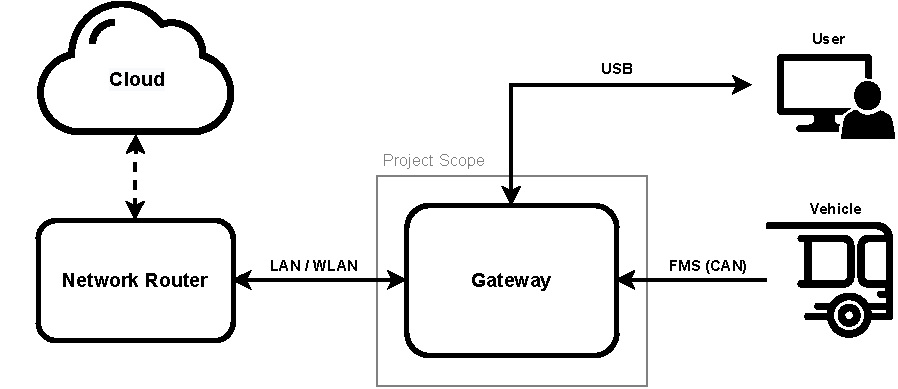
\includegraphics[width=9cm]{images/Block_Diagram}
	\caption{System Block Diagram}
	%\vspace{-2ex}
	%\caption*{\textbf{Source:} Original task definition}
	\label{fig:constellation_HW}
\end{figure}

FMS-Packages are received by the gateway and then get redirected to a local server application, running on the vehicles on-board network router.
Further, the information can be transmitted over the internet to a cloud-based system.

\begin{itemize}
	\item bla 1
	\item bla 2
	\item bla 3
\end{itemize}

Various use cases were defined in \cref{sec:use_cases}.
	\newpage
\section{Product Requirements}
\subsection{Protocols and Interfaces}
blabla

\subsection{Hardware}
The on purpose build, custom hardware contains all necessary components integrated on a single printed circuit board (PCB).
The core is based on a micro controller of the ESP32-Family. 



\subsection{Firmware}
For all use cases defined in \cref{sec:use_cases}, 

\subsection{Web Server Communication Tool}
The web server communication tool is the sole device communicating with the hardware. The system has the following requirements:
\begin{itemize}
        \item The web server shall be written in Python.
        \item The system shall handle http request to achieve a good communication between the embedded system and the host.
        \item The system shall store the streamed data and make it available for further processing.
        \item The system should host files for the hardware (e.g. configuration files, firmware updates).
\end{itemize}

\subsection{Data Interpreter and Visualizer}
This Python-based tool consists of two separated parts and follows the subsequent requirements:

\begin{itemize}
		\item The Data Interpreter shall parse FMS-Packages and prepares them for further usage.
		\item The Data Visualizer shall use a Graphical User Interface (GUI) in order to present the FMS data (e.g. parameter values).
\end{itemize}
	\newpage
\section{Use Cases}
\label{sec:use_cases}
\subsection{UC1 Driving Quality Analysis}
Having a clear understanding of a drivers behavior, is very important for fleet operators. Having data about the vehicle operators can lead to less emissions, improve customer satisfaction and improve the drivers behavior. Our system can be deployed to gather driving data in a very detailed manner.
The \acrlong{imu} provides accurate motion data of the vehicle, which leads to a better understanding of the driving performance.

\subsection{UC2 Vehicle Maintenance Report}
Managing a large fleet of vehicles requires enormous effort. In order to minimize down time it is important to preemptively warn about upcoming and present issues. Our system makes it possible to gather continuous information about the status of the fleet without physical access. 

\subsection{UC3 Real Time Telemetry Data}
Most of modern vehicles are already equipped with \acrshort{gnss} receivers for providing location updates to the \acrlong{fms}. However it is difficult to differentiate if a vehicle is currently parked or just slowly moving (e.g. due to traffic jams). With the help of knowing the exact driving velocity, a better prediction of potential arrival time can be achieved. Additional data, like the state of passenger doors can directly inform the system about a potential delay of departure.
	\input{sections/5_project_schedule}
	

% % % % % % % % % % % % % % % % % % % % % % % % % % % % % % % %
% ANHANG
% % % % % % % % % % % % % % % % % % % % % % % % % % % % % % % %
\appendix


%Nummerierung wieder auf roemisch umschalten

%\newpage
%\section{References}
%\label{anx:ref}
%% Do not repeat items covered in other documents or in a global project definitions and acronyms document
%\renewcommand{\refname}{} %kein Titel vor Literaturverzeichnis
%\vspace{-1.2cm}
%\bibliographystyle{ieeetr} %Literatur durchnumerieren
%\bibliography{lit}
%\nocite{*} %Alle Literatur aufführen
	
\end{document}